% Drugi del predavanja: od široke prosojnice nasveta 4 do slabe prosojnice
% nasveta 6, v temi Berlin in razmerju 16 : 9. O razdelitvi na tri dokumente
% glej stevilke.tex, o zgradbi predavanja pa berlin-4-3.tex.
\documentclass[aspectratio=169]{beamer}
\usepackage[utf8]{inputenc}
\usepackage[T1]{fontenc}
\usepackage[slovene]{babel}
\usepackage{amsmath}
\usepackage{minted}
\usepackage{tikz}
\usetikzlibrary{decorations.pathreplacing}
\usetheme{Berlin}
% Predavanje je razdeljeno na tri dokumente, ker se tema in razmerje sredi
% dokumenta ne dasta zamenjati: berlin-4-3.tex, berlin-16-9.tex in
% prosojnice.tex, ki prva dva vključi. Številke prosojnic se nadaljujejo iz
% dokumenta v dokument: ob koncu dokument zapiše zadnjo številko v datoteko
% ⟨ime⟩.stevec, naslednji pa jo prebere z \input{⟨ime⟩.stevec}. Dokumente zato
% prevajajte po vrsti.
\makeatletter
\AtEndDocument{%
  \newwrite\stevec
  \immediate\openout\stevec=\jobname.stevec
  \immediate\write\stevec{\string\setcounter{framenumber}{\the\c@framenumber}}%
  \immediate\closeout\stevec
}
\makeatother


\title{Predstavitve}
\author{Računalniški praktikum}

% Pomanjšana prosojnica iz teme.pdf: prvi argument je stran, drugi ime teme.
\newcommand{\tema}[2]{%
  \begin{minipage}[t]{0.32\textwidth}
    \centering
    \fbox{\includegraphics[page=#1, width=0.95\textwidth]{teme}}\\[-0.5ex]
    {\tiny #2}
  \end{minipage}%
}

\begin{document}
\input{berlin-4-3.stevec}

% Ista prosojnica kot na koncu berlin-4-3.tex, zdaj v širokem formatu in le z
% zadnjim korakom, saj je slika že zgrajena.
\newcommand{\vsotakoraki}{4}
% Dva dokaza formule za vsoto prvih n števil. Prosojnico vključita
% berlin-4-3.tex, kjer je utesnjena, in berlin-16-9.tex, kjer je najprej še z
% glavo in nogo, nato pa brez njiju. Dokument mora naložiti paketa amsmath in
% tikz s knjižnico decorations.pathreplacing ter z ukazom \vsotakoraki določiti,
% katere korake prosojnice pokaže: v berlin-4-3.tex vse (1-), v
% berlin-16-9.tex le zadnjega (4), saj se tam slika ne gradi več.
\begin{frame}<\vsotakoraki>{V matematiki so slike sploh pomembne}
  \begin{columns}[T]
    \begin{column}{0.48\textwidth}
      \begin{block}{Indukcija}
        \scriptsize
        % Razmik okoli izpeljave ostane sicer takšen kot pri običajni velikosti.
        \setlength{\abovedisplayskip}{3pt}
        \setlength{\belowdisplayskip}{3pt}
        Trdimo, da za vsak \(n \geq 1\) velja
        \(1 + 2 + \dots + n = n(n + 1)/2\).

        \emph{Baza.} Za \(n = 1\) je leva stran \(1\), desna pa
        \(1 \cdot 2/2 = 1\).

        \emph{Korak.} Predpostavimo, da formula velja za \(n\). Po indukcijski
        predpostavki je
        \begin{align*}
          &1 + \dots + n + (n + 1)
          = \frac{n(n + 1)}{2} + (n + 1) \\
          &= \frac{n(n + 1) + 2(n + 1)}{2}
          = \frac{(n + 1)(n + 2)}{2},
        \end{align*}
        kar je formula za \(n + 1\). Po načelu indukcije formula velja za vsak
        \(n \geq 1\).
      \end{block}
    \end{column}
    \begin{column}{0.48\textwidth}
      \begin{block}{Slika}
        \centering
        % Modro stopnišče je 1 + 2 + 3 + 4, rdeče je enako, le obrnjeno. Skupaj
        % dasta pravokotnik n × (n + 1).
        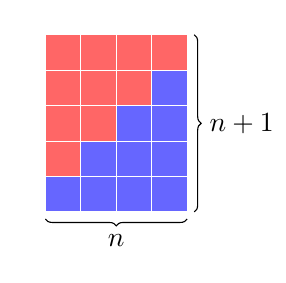
\begin{tikzpicture}[x=0.45cm, y=0.45cm]
          \useasboundingbox (-0.5, -1.2) rectangle (6, 5.2);
          \foreach \i in {1, ..., 4}
            \foreach \j in {1, ..., \i}
              \fill[blue!60, draw=white] (\i - 1, \j - 1) rectangle ++(1, 1);
          \foreach \i in {1, ..., 4}
            \foreach \j in {\i, ..., 4}
              \fill<2->[red!60, draw=white] (\i - 1, \j) rectangle ++(1, 1);
          \draw<3->[decorate, decoration={brace, mirror}] (0, -0.2) -- (4, -0.2)
            node[midway, below=2pt] {\(n\)};
          \draw<3->[decorate, decoration={brace, mirror}] (4.2, 0) -- (4.2, 5)
            node[midway, right=2pt] {\(n + 1\)};
        \end{tikzpicture}

        \onslide<4->{\(2 (1 + \dots + n) = n (n + 1)\)}
      \end{block}
    \end{column}
  \end{columns}
\end{frame}


\setbeamertemplate{navigation symbols}{}
\setbeamertemplate{headline}{}
\setbeamertemplate{footline}[page number]
\setbeamertemplate{page number in head/foot}[framenumber]

% Ista prosojnica kot na začetku tega dokumenta, zdaj brez glave in noge.
% Dva dokaza formule za vsoto prvih n števil. Prosojnico vključita
% berlin-4-3.tex, kjer je utesnjena, in berlin-16-9.tex, kjer je najprej še z
% glavo in nogo, nato pa brez njiju. Dokument mora naložiti paketa amsmath in
% tikz s knjižnico decorations.pathreplacing ter z ukazom \vsotakoraki določiti,
% katere korake prosojnice pokaže: v berlin-4-3.tex vse (1-), v
% berlin-16-9.tex le zadnjega (4), saj se tam slika ne gradi več.
\begin{frame}<\vsotakoraki>{V matematiki so slike sploh pomembne}
  \begin{columns}[T]
    \begin{column}{0.48\textwidth}
      \begin{block}{Indukcija}
        \scriptsize
        % Razmik okoli izpeljave ostane sicer takšen kot pri običajni velikosti.
        \setlength{\abovedisplayskip}{3pt}
        \setlength{\belowdisplayskip}{3pt}
        Trdimo, da za vsak \(n \geq 1\) velja
        \(1 + 2 + \dots + n = n(n + 1)/2\).

        \emph{Baza.} Za \(n = 1\) je leva stran \(1\), desna pa
        \(1 \cdot 2/2 = 1\).

        \emph{Korak.} Predpostavimo, da formula velja za \(n\). Po indukcijski
        predpostavki je
        \begin{align*}
          &1 + \dots + n + (n + 1)
          = \frac{n(n + 1)}{2} + (n + 1) \\
          &= \frac{n(n + 1) + 2(n + 1)}{2}
          = \frac{(n + 1)(n + 2)}{2},
        \end{align*}
        kar je formula za \(n + 1\). Po načelu indukcije formula velja za vsak
        \(n \geq 1\).
      \end{block}
    \end{column}
    \begin{column}{0.48\textwidth}
      \begin{block}{Slika}
        \centering
        % Modro stopnišče je 1 + 2 + 3 + 4, rdeče je enako, le obrnjeno. Skupaj
        % dasta pravokotnik n × (n + 1).
        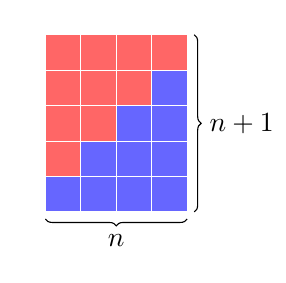
\begin{tikzpicture}[x=0.45cm, y=0.45cm]
          \useasboundingbox (-0.5, -1.2) rectangle (6, 5.2);
          \foreach \i in {1, ..., 4}
            \foreach \j in {1, ..., \i}
              \fill[blue!60, draw=white] (\i - 1, \j - 1) rectangle ++(1, 1);
          \foreach \i in {1, ..., 4}
            \foreach \j in {\i, ..., 4}
              \fill<2->[red!60, draw=white] (\i - 1, \j) rectangle ++(1, 1);
          \draw<3->[decorate, decoration={brace, mirror}] (0, -0.2) -- (4, -0.2)
            node[midway, below=2pt] {\(n\)};
          \draw<3->[decorate, decoration={brace, mirror}] (4.2, 0) -- (4.2, 5)
            node[midway, right=2pt] {\(n + 1\)};
        \end{tikzpicture}

        \onslide<4->{\(2 (1 + \dots + n) = n (n + 1)\)}
      \end{block}
    \end{column}
  \end{columns}
\end{frame}


% Ista prosojnica v šestih Beamerjevih temah. Slike so izvožene iz zbornice,
% predavanja/08-predstavitve/izvoz.sh.
\begin{frame}{Beamerjeve privzete teme imajo veliko odvečnih elementov}
  \centering
  \tema{1}{Madrid}\hfill\tema{2}{Warsaw}\hfill\tema{3}{AnnArbor}

  \medskip
  \tema{4}{Antibes}\hfill\tema{5}{PaloAlto}\hfill\tema{6}{Darmstadt}
\end{frame}


\begin{frame}[fragile]{Odstranite odvečne privzete nastavitve}
  \begin{minted}[fontsize=\footnotesize]{latex}
\setbeamertemplate{navigation symbols}{}
\setbeamertemplate{headline}{}
\setbeamertemplate{footline}[page number]
\setbeamertemplate{page number in head/foot}[framenumber]
  \end{minted}
\end{frame}

\end{document}
